%%%%%%%%%%%%%%%%%%%%%%%%%%%%%%%%%%%%%%%%%%%%%%%%%%%%%%%%%%%%%%%%%%%%%%%%%%%%%%%
%
% Tommy P. Keane
% Master of Science Thesis
% Department of Electrical and Microelectronic Engineering
% Rochester Institute of Technology
%
% April 2011
%
%
%
% Funded By: Lenel Systems Inc., A UTC Fire & Security Corporation
%
% Algorithm Intellectual Property Owned By: Lenel Systems Inc.
%
%
% http://www.tommypkeane.com
%
%%%%%%%%%%%%%%%%%%%%%%%%%%%%%%%%%%%%%%%%%%%%%%%%%%%%%%%%%%%%%%%%%%%%%%%%%%%%%%%

%%%%%%%%%%%%%%%%%%%%%%%%%%%%%%%%%%%%%%%%%%%%%%%%%%%%%%%%%%%%%%%%%%%%%%%%%%%%%%%
%
% CHAPTER 2
%
% SECTION 3: Histograms and Color Imagery
%
%%%%%%%%%%%%%%%%%%%%%%%%%%%%%%%%%%%%%%%%%%%%%%%%%%%%%%%%%%%%%%%%%%%%%%%%%%%%%%%


%%%%%%%%%%%%%%%%%%%%%%%%%%%%%%%%%%%%%%%%%%%%%%%%%%%%%%%%%%%%%%%%%%%%%%%%%%%%%%%
% BEGIN DOCUMENT

A digital image histogram \cite{Gonzalez2008}, referred to by $\bf{h}(\bf{n})$, is a discrete function (a vector) that represents intensity value totals (counted) from the related digital image, and whose independent variable ($\bf{n}$, a vector) represents the center value of the subset of intensities from the related digital image, called the \textbf{bin center}. The bin is described by its center value ($n_{i}$) and its width ($r$), as existing in the interval in Eq. \ref{histBin}. Thus, an intensity histogram is a vector holding the total number of intensity values in the intervals related to the indices of that vector.

\begin{equation}
\label{histBin}
\left[n_{i}-\frac{r}{2},n_{i}+\frac{r}{2}\right)
\end{equation}

Harkening back to our assumption of single channel images with 8-bits per pixel (8-bpp), this allows for a maximum of 256 unique intensity values per pixel. And again these intensity values are assumed to be statistically random over the 2-D spatial domain of the image. So for a single channel image with 8-bpp, a 256 bin histogram can be developed with integer width bins (corresponding to pixel locations) with a total intensity range of $[0,255]$ with bin intervals: $[n_{i},n_{i+1}) \quad \forall n_{i} \in \{\mathbb{Z}\}_{0}^{255}$. This histogram is again labeled $\textbf{h}(\textbf{n})$ and mathematically the centers can be assumed to be at $\frac{n_{i+1}-n_{i}}{2}$ with width $r=1$, although in practice the half values are outside the 8-bpp intensity range, so vector $\bf{n}$ is understood as $\bf{n}=\begin{bmatrix}0&1&2&\cdot\cdot\cdot&255\end{bmatrix}^{T}$. The total sum of that histogram, as shown in Eq. \ref{histSum}, is the product of the image dimensions, $\mathfrak{m} \cdot \mathfrak{n}$, provided the bins cover the full intensity range as developed here. (Note: histograms are one-to-one transformations of the image data, meaning that no pixel is counted in the histogram more than once, by definition.)

\begin{equation}
\label{histSum}
	\mathfrak{m} \cdot \mathfrak{n} = \sum_{i=0}^{255}{h(n_{i})}
\end{equation}

As stated, any digital image histogram that covers the entire image and the entire intensity range will always sum to the image size, because all intensity values will fall in the range of the histogram bin intervals, by construction, and can only be counted once, by definition. This is how the PMF can be constructed; by normalizing a histogram by its sum total. The normalization will impose the constraint that an image's intensity histogram's sum will equal 1, which is a condition of a PMF \cite{Papoulis2002}; and clearly the histogram describes how many pixels correspond to an intensity value or range, which when normalized can be seen as a corollary to the probability of that intensity value or range of intensities occurring within the image. The specificity of the histogram to the image must be recognized though; because what the histogram conveys is that the pixels in \textit{this} image are distributed in \textit{these} amounts. Since an image is only being modeled as a random variable its normalized histogram is not identical to a PMF, because it is a descriptor of a specific instance of a random variable (the image formation) not a general descriptor of the random variable for that experiment. The imaging equivalence made here is that the normalized histogram is cognitively generalized to be a descriptor of the image, and is the approximation of the descriptor of the real-world scene that the related image has captured. This is a very important point of consideration, but its detailed discussion has been deferred to the next section of this chapter and it should be taken for now as an assumption of this development.

\begin{figure}[h]
\centering
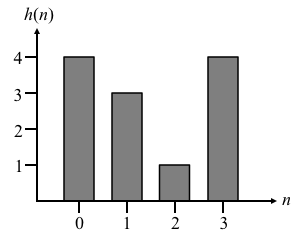
\includegraphics[width=.5\textwidth]{sampleHistogram}
\caption{Example Intensity Histogram}
\label{sampleHist}
\end{figure}

After understanding what a histogram is and how to build it, its use is only as good as its limitations. And one of the most important limitations of an intensity histogram is the loss of spatial information in its generation. No spatial information is mathematically present in the calculation of a basic intensity histogram, as it has been described and used herein. However, through basic knowledge related to the structure and generation of images, there can be some simple yet significant spatial information extracted cognitively from a digital histogram. To illustrate this concept Figure \ref{sampleHist} displays a very simple histogram for a 2-bpp image of size $3\times4$.

\begin{figure}[h]
\centering
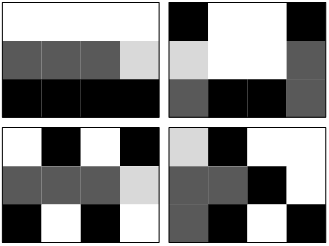
\includegraphics[width=.6\textwidth]{sampleImages}
\caption{Example 2-bpp Images with Identical Intensity Histograms (0 to 3 :: Black to White)}
\label{sampleIm}
\end{figure}

What is gathered from this histogram about the image is that there are equal numbers of extreme intensity values, and much more 1s than 2s (here the indices correspond to the intensity values as it is a full-range histogram). This results from a simple reading of the histogram and understanding its basic construction. But in terms of image information, it is also quite clear that this is a mostly dark image with high contrast. This comes from examining the values and structure of the histogram. The values are not bunched up nor are they spread evenly across intensities, so there are some significant edges in the image. Again, though, there is no explicit orientation information present in the mathematical construction of a histogram. Implicitly though this absolutely cannot be a smooth intensity gradient image, meaning that there is no way to construct these pixels with these values so that there is no edge with a transition greater than 1. Figure \ref{sampleIm} shows 4 unique images that all share the histogram shown in Figure \ref{sampleHist}. For more on contrast and image analysis through histograms, refer to \cite{Gonzalez2008}.


These images come from the set of 138,600 possible images $\left(\frac{12!}{4!\cdot3!\cdot1!\cdot4!}\right)$ that share the histogram in Figure \ref{sampleHist}. But this is just a purely mathematical example with no constraints. By the nature of reality, such as the spatial and temporal continuity of objects within reality, images of real scenes are highly constrained subset of all the possible images from the total set (all the possible combinations of intensities given the number of pixels in the image). Any 2-bpp image of size $3\times4$ is actually in the general set of $4^{12}$ images, and so the set of images with the histogram in Figure \ref{sampleIm} is roughly less than $0.8\%$ of the total set, while still unconstrained to real world shapes. Extending this idea to the images used in this algorithm, which were all roughly of the size $480 \times 640$ and were 3 channel images of 8-bpp, that gives 768 possible values per pixel location ($3\cdot2^{8}$). This means that there are $768^{480\cdot640}$ possible images of this size with no spatial or histogram constraint. Any histogram, color constancy model, texture, object contiguity, or any other real world aspect or feature relevant to the digital image will create a smaller and smaller subset. Yet, a rigorous mathematical comparison is not applicable here, because the purpose here is to illuminate how large the set of all possible images is, and how small the subset of all possible real world images is, and then how much smaller the set of all similar images is, and ultimately how much smaller the set of similar real world images with similar histograms is. There are several layers of practical and mathematical restrictions creating such a small subset to create an image of a real scene that captures its content accurately. Clearly it is not much of a theoretical stretch, despite the lack of the explicit mathematics, to determine that the approximation of using a normalized histogram to produce the PMF of an image is a theoretically relevant and an apt, realistic association. Conceptually what is being stated or assumed is that when viewing the same scene, two different views will be sampling the same random function, meaning that they should be describable by the same PMF in the overlap region. As the overlap decreases between the views, the scene being captured is varying more and more, between the views, as parallax and occlusions begin to occur. The assumption that this is a small set of possible images since they are viewing the same scene is still valid; but the assertion that the views are still observing the same scene begins to fall apart. The scene PDF for each view is becoming more and more distinct, and as the PDF is understood to describe the view of the scene (the random variable), the portions that overlap in the imaged views are becoming less and less dependent upon one another. The PMFs of each view in the overlap as the cameras are rotated or separated by significant amounts become more independent and thus more separable and their possible mutual information decreases (as will be discussed in the next section). It will be shown as a major characteristic of the evaluation of this algorithm and its robustness, to understand what factors and scenarios are crippling or limiting in terms of asserting dependence between the distinct views' PMFs.


An interesting note in the development of the PMFs is in terms of the amount and variation in the data in the image. As $\mathfrak{m}$ and $\mathfrak{n}$ decrease there is less opportunity for variation or consistency in the image, depending upon the value of $b$ (the bit-depth). If $2^{b}$ is significant (\ie not much, much less) compared to $\mathfrak{m} \cdot \mathfrak{n}$, then each instance of an image from that theoretical set can have significant variation. This could even allow for significant variation between views are capturing the same exact scene or sections of the views are capturing the same exact scene (spatio-temporally). This is a crippling limit of these assumptions and a source of our empirically derived overlap requirement for the algorithm, as will be discussed in Chapter 4.


These are extremely important characteristics to understand about intensity histograms. It will be discussed in Chapter 3 as to how computationally taxing the histogram calculation is, and expanding it (especially to the full intensity range) is a significant detriment to the algorithm. This all follows directly into the generation of, and ambiguities inherent to, mutual information calculations of digital images. So first it is necessary to take a similar look at the calculation of mutual information, and what it can and will represent in this context.


%%%%%%%%%%%%%%%%%%%%%%%%%%%%%%%%%%%%%%%%%%%%%%%%%%%%%%%%%%%%%%%%%%%%%%%%%%%%%%%
% END OF DOCUMENT

